% Appendix A

\appendix
\renewcommand{\thechapter}{A}
\chapter{SIGMUND, manual de uso} % Main appendix title

\label{APP_SIGMUNDMAN} % For referencing this appendix elsewhere, use \ref{AppendixA}

\section*{Introducción}

La aplicación \texttt{SIGMUND} permite llevar a cabo simulaciones del modelo dinámico descrito en el capítulo \ref{chapterDINAMICA}, tanto de forma interactiva como en modo \texttt{batch}.

El \textit{software} se ha desarrollado en \texttt{Python} y puede ejecutarse en cualquier entorno que disponga de la versión \texttt{3.} o superior. Se recomienda instalar una distribución que incluya todos los paquetes habituales en cálculo científico. En concreto, la distribución \href{https://www.continuum.io/}{Anaconda} proporciona un entorno completo sobre el que instalar \texttt{SIGMUND} sin necesidad de añadir manualmente ningún paquete adicional.

El paquete se instala desde \texttt{github} clonando el repositorio:

\fontsize{3.5mm}{3.5mm}\selectfont
\begin{verbatim}
 clone https://github.com/jgalgarra/sigmund 
\end{verbatim}
\normalsize

Este manual describe la aplicación en su versión \texttt{2.05}.
 
\subsection*{Formato de los ficheros de entrada}
\label{sec:ASIGMUNDMAN_input_file_format}

Las simulaciones requieren dos ficheros de entrada para cada red, que se almacenan en el directorio \path{sigmund/src/pak_tfm/input}. El primero se llamará \texttt{XXX\_a.txt} donde \textit{XXX} puede ser cualquier nombre, lo único obligatorio es que termine en \texttt{\_a.txt}. El segundo debe llamarse \texttt{\_b.txt}. Por motivos de simplicidad, la interfaz de usuario se refiere a plantas y polinizadores, pero puede usarse para otros tipos de red mutualista.
El primer fichero contiene los coeficientes de la matriz de adyacencia en el sentido polinizador - planta, esto es, el beneficio mutualista que la presencia de cada individuo del polinizador $i$ supone para la planta $j$. Los datos se organizan en columnas, cada una de ellas correspondiente a una especie de planta, en modo texto y separados por tabuladores. Hay una fila por cada especie de polinizador y cuatro adicionales con la población inicial de la especie de planta, el coeficiente $c_{j}$ (fórmula \ref{eq:alphavariable}), el término de fricción intraespecífica $\alpha_{j}$ y las tasas vegetativas de nacimiento y muerte.

En el fichero \texttt{\_b} se almacena la información en el sentido planta - polinizador, con tantas columnas como especies de estos segundos haya.

\begin{figure}[h!]
\centering
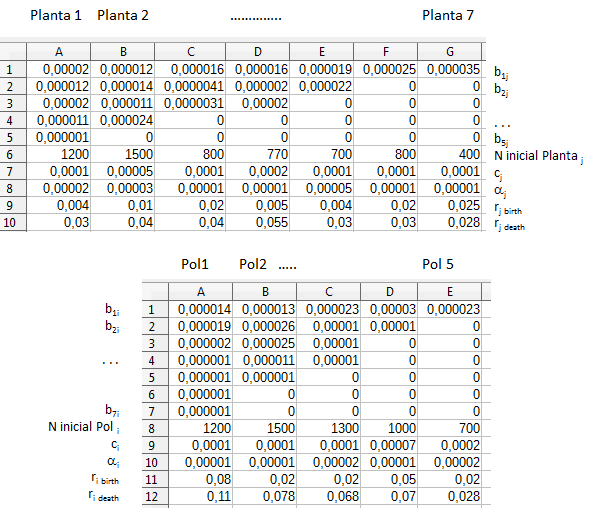
\includegraphics[scale=1]{ManFigs/matricessim.png}
\caption{Ejemplo de ficheros de entrada para la simulación de la figura \ref{fig:DINAMICA_SAT_exper_resilience_strong}.}
\label{fig:ASIGMUNDMAN_matricessim}
\end{figure}

\clearpage
\subsection*{Uso interactivo}
\label{sec:ASIGMUNDMAN_ui}

$SIGMUND$ queda preparado para funcionar una vez clonado el repositorio. Navegar hasta el directorio \path{sigmund/src/pak_tfm} que se habrá creado en ese proceso. Si se utiliza \texttt{Windows} hágase doble click con el botón izquierdo sobre el icono \texttt{sigmund\_tool.py}. Bajo \texttt{Linux} se puede lanzar con el comando \texttt{sigmund\_tool.py}.

Aparecerán dos ventanas, una con la salida de la sesión \texttt{Python} y otra con la interfaz de usuario de \texttt{SIGMUND}. La primera puede redirigirse a un fichero o hacia donde el usuario considere conveniente.


\begin{figure}[h!]
\centering
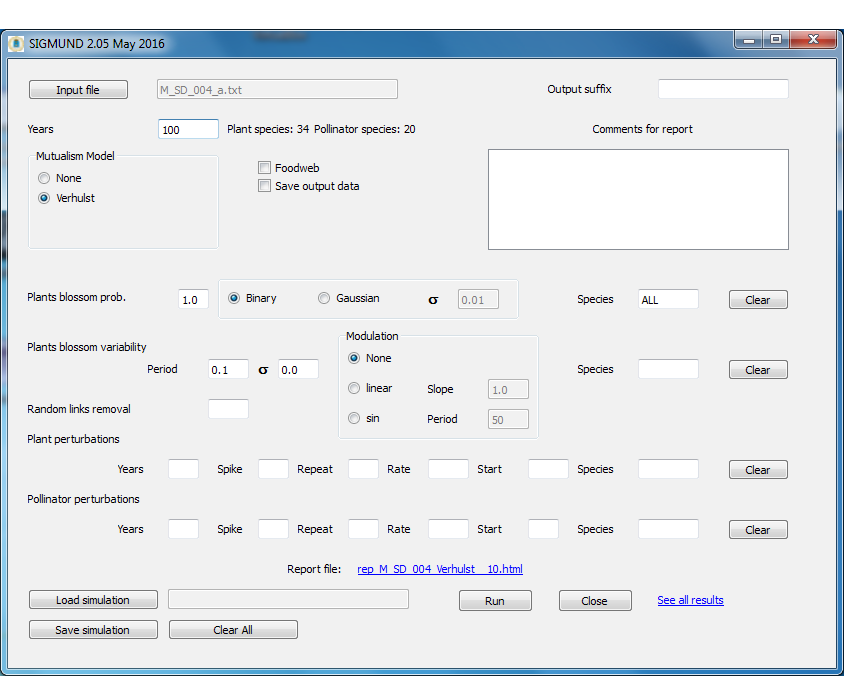
\includegraphics[scale=1]{ManFigs/sigmund_ui.png}
\caption{Interfaz de usuario de \texttt{SIGMUND} }
\label{fig:ASIGMUNDMAN_matricessim}
\end{figure}

La interfaz de usuario está construida con el entorno gráfico \texttt{Qt} por lo que la apariencia puede variar ligeramente dependiendo del sistema operativo y del juego de fuentes instalado. 

Esta es la función de los distintos campos de entrada.

\begin{itemize}
\item \texttt{Input File}: nombre de cualquiera de los ficheros de configuración de la red almacenados en \path{./input}. Se puede escoger de forma manual o se cargará automáticamente si se recrea una simulación almacenada. La interfa de usuario mostrará el número de especies de cada clase.

\item \texttt{Years}:  Duración de la simulación en años, obligatorio.

\item \texttt{Output suffix}: sufijo de salida opcional que se añadirá al nombre de los ficheros de salida que se escriben en  \path{./output}.

\item \texttt{Comments}: campo opcional de escritura libra que sirve, por ejemplo, para que una descripción del experimento se pueda guardar en el informe de ejecución.

\item \texttt{Mutualism Model}: indica si se usa el modelo de Verhuslt modificado o no hay mutualismo.

\item \texttt{Food web}: indica si hay una \textit{food web} actuando la comunidad mutualista.

\item \texttt{Save output data}: indica si se quieren guardar los resultados numéricos de la simulación en ficheros de texto. Debido a que la simulación se calcula día a día el tamaño de estos ficheros puede ser muy grande y se ralentizará la simulación.

\end{itemize}

El sistema puede atacarse de manera opcional con distintos tipos de perturbaciones:
\begin{itemize}
\item \texttt{Random links removal}: porcentaje de enlaces de la red que se retiran de manera aleatoria.

\item \texttt{Plants blossom probability}: Probabilidad de florecimiento. 

\begin{itemize}
	\item \texttt{Binary}: la floración de cada año se trata como un experimento de Bernouilli. Las especies indicadas en la lista florecen con la intensidad habitual o no lo hacen en absoluto.

    \item \texttt{Gaussian}: se modula la intensidad con una normal de media igual al parámetro de probabilidad y desviación estándar igual a $\sigma$.
    
    \item \texttt{Species}: lista de especies afectadas que puede ser un rango con formato \texttt{Python}, por ejemplo 1:3, una lista de números separados por comas o una combinación de ambos. El valor \texttt{ALL} indica que todas las especies sufren la perturbación.
\end{itemize}

\item \texttt{Plants blossom variability}: Variabilidad de la floración debida a la falta de coincidencia en el tiempo de la floración con la actividad animal.
\begin{itemize}
	\item \texttt{Period}: Fracción del año en que coinciden floración y actividad animal, modelada según una gaussiana.

    \item \texttt{Deviation}: Desviación estándar del periodo de floración.
    
    \item \texttt{Type}:  \texttt{None} media constante, \texttt{linear} media vairable definida por la pendiente o \texttt{sinusoidal} media variable definida por el periodo.
    
    \item \texttt{Species}: lista de especies afectadas.
\end{itemize}

\end{itemize}

Perturbaciones externas. Ataques exógenos (epidemias, sequías, migraciones...) que pueden producir un aumento abrupto de las tasas
de mortalidad. Hay dos líneas de entrada, una para plantas y otra para animales.

\begin{itemize}
 \item \texttt{Years}: Duración de la perturbación en años.
 \item \texttt{Spike}: Fracción activa del periodo de perturbación. Util en caso de perturbación repetitiva.
 \item \texttt{Spike}: Aumento de la tasa de mortalidad expresado en fracción unitaria.
 \item \texttt{Start}: Año de la simulación en que la perturbación empieza a tener efecto.
 \item \texttt{Species}: lista de especies afectadas.
\end{itemize}

Por último, los parámetros de una simulación pueden salvarse en fichero y recuperarse posteriormente con:
\begin{itemize}
 \item \texttt{Load simulation}
 \item \texttt{End simulation}
\end{itemize}

\subsection*{Ejemplos}

En esta sección se presentan distintos casos de uso con el simulador y su significado ecológico.

\begin{figure}[h!]
\centering
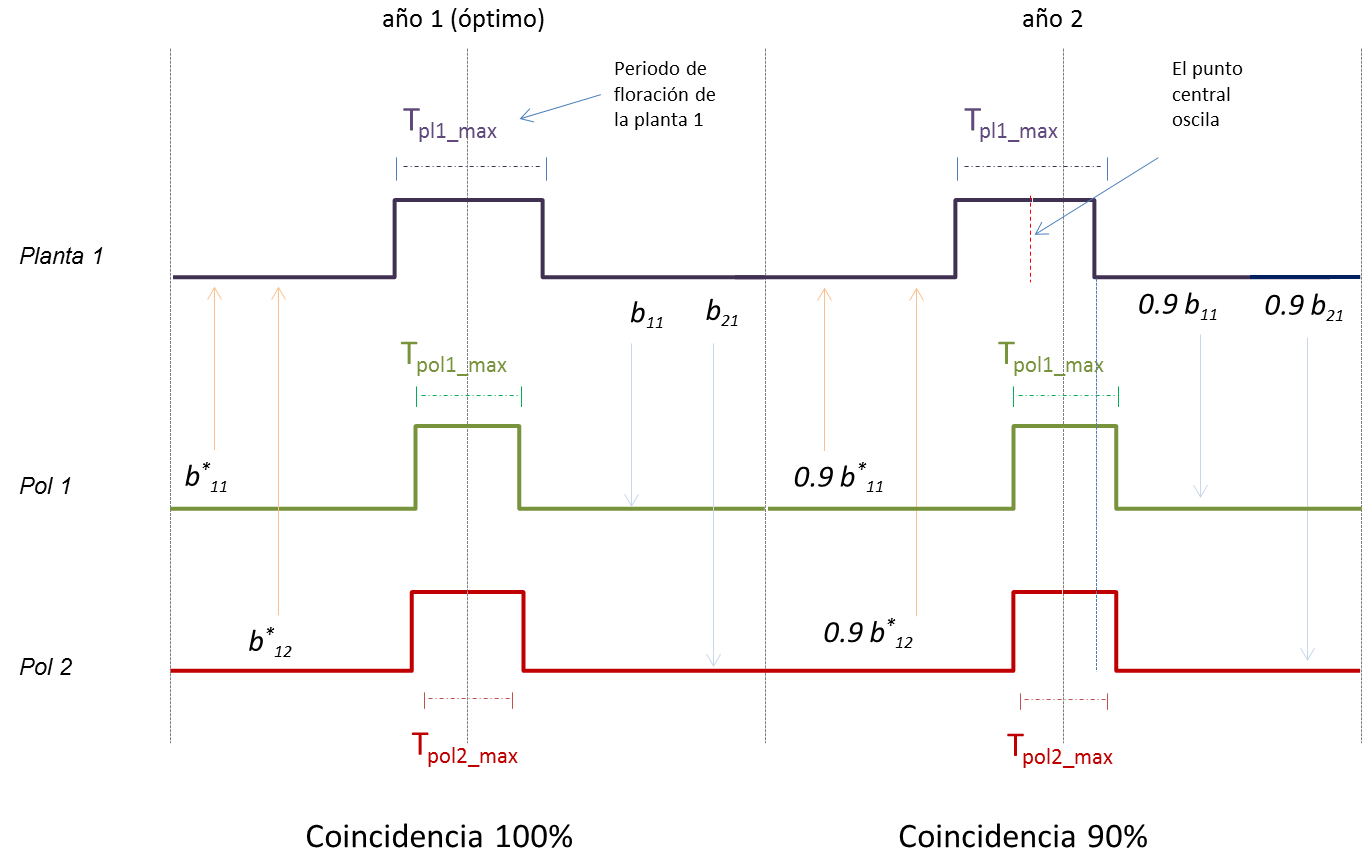
\includegraphics[scale=1]{ManFigs/sigmund_tiempos.png}
\caption{Significado de la coincidencia del periodo de floración}
\label{fig:ASIGMUNDMAN_sigmund_tiempos}
\end{figure}

En la figura \ref{fig:ASIGMUNDMAN_sigmund_tiempos} se ha representado el modelo simplificado que se emplea para el periodo de floración. El primer año, el periodo de floración de las
plantas y de los animales coincide al $100\%$ con el de estos últimos, por lo que el beneficio mutualista es óptimo y loa coeficientes planta polinizador son los que se leen de la
matriz de interacción. El segundo año, el periodo de floración se ha adelantado y el área de coincidencia es solo el $90\%$ del óptimo de manera que los coeficientes se multiplicarán
por este factor reductor en la simulación.

\begin{figure}[h!]
\centering
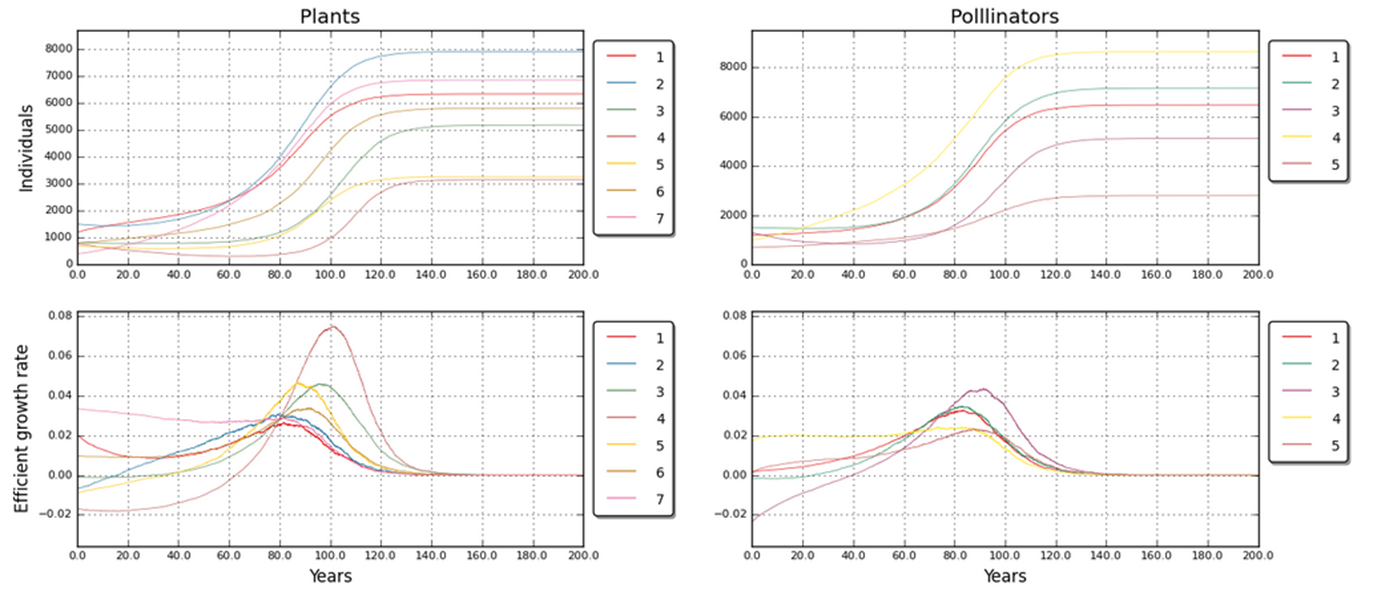
\includegraphics[scale=1]{ManFigs/sigmund_red_exper.png}
\caption{Evolución dinámica sin perturbaciones en una red de ejemplo.}
\label{fig:ASIGMUNDMAN_sigmund_red_exper}
\end{figure}

\begin{figure}[h!]
\centering
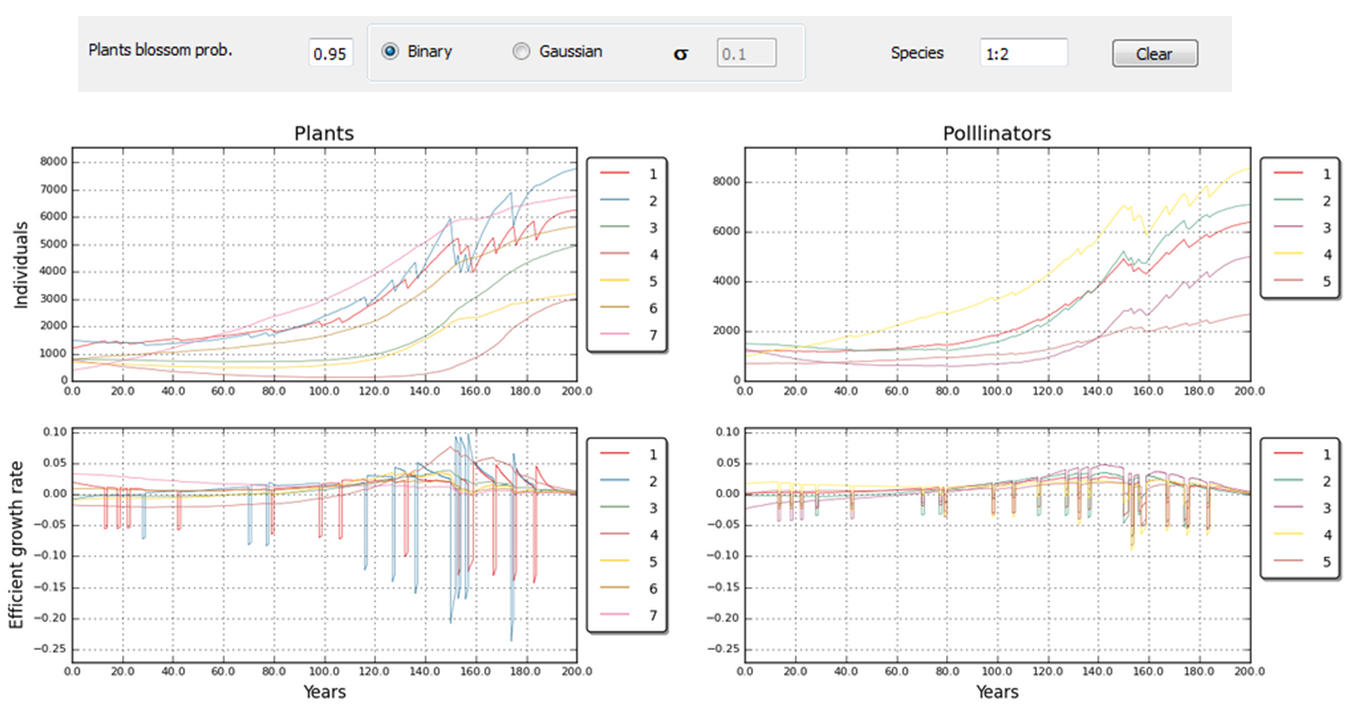
\includegraphics[scale=1]{ManFigs/sigmund_oscilacion_intensidad.png}
\caption{Perturbación binaria de la intensidad de floración.}
\label{fig:ASIGMUNDMAN_sigmund_oscilacion_intensidad}
\end{figure}

\clearpage
En las dos figuras precedentes se ve la evolución dinámica de una pequeña red ficticia. En la primera se ve como las especies crecen hasta alcanzar el punto de equilibrio de poblaciones máximas en ausencia de perturbaciones. En la segunda, se incluye una variación de la intensidad de la floración en las dos especies de planta más generalistas, la $1$ y las $2$. El tipo de perturbación es binaria y la probabilidad es $0.95$, así que, por término medio, el $95\%$ de los años la floración es normal y el $5\%$, inexistente. Puede observarse la caída abrupta de las tasas
de crecimiento eficiente de ambas especies de plantas cuando ocurre uno de estos eventos. Esto afecta a los polinizadores y el sistema trada más tiempo en alcanzar las poblaciones máximas.

\begin{figure}[h!]
\centering
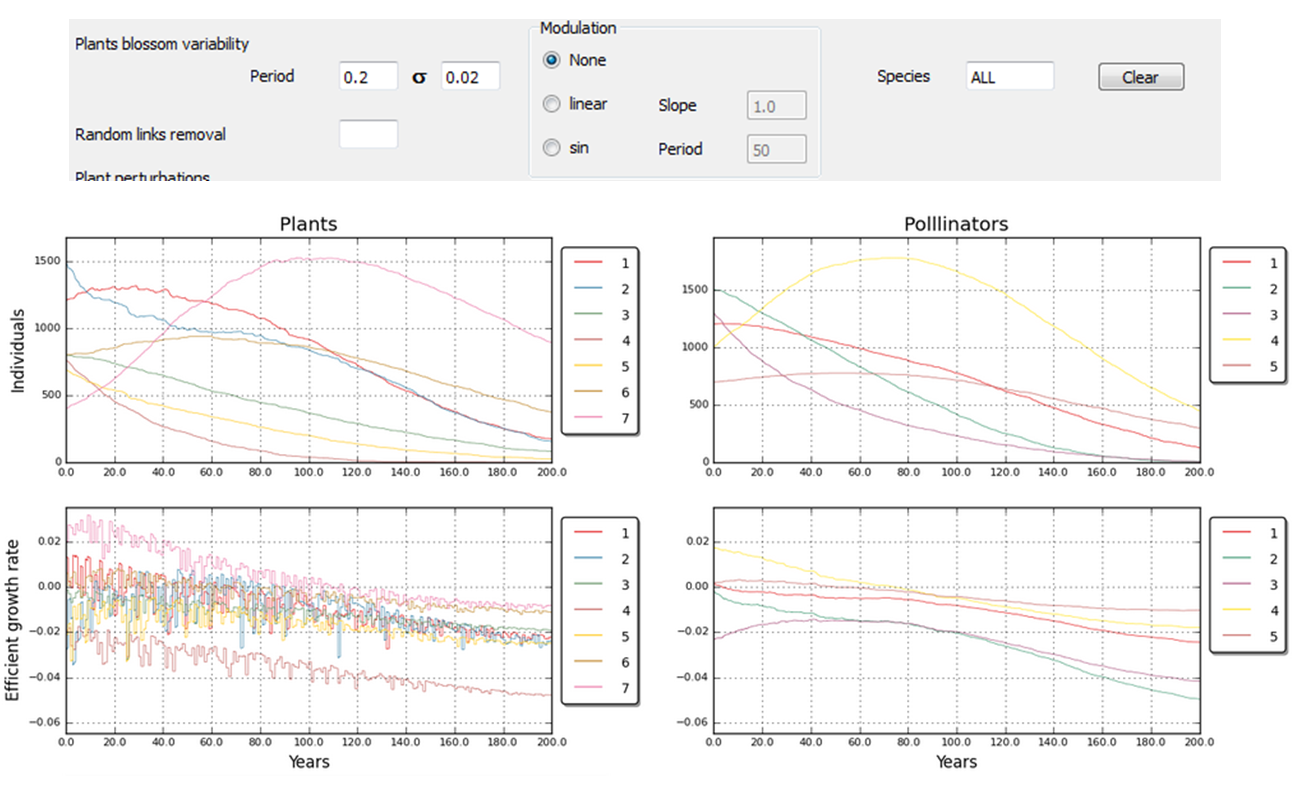
\includegraphics[scale=1]{ManFigs/sigmund_oscilacion_tiempo_none.png}
\caption{Perturbación gaussiana en el periodo de floración.}
\label{fig:ASIGMUNDMAN_sigmund_oscilacion_tiempo_none}
\end{figure}

En la figura \ref{fig:ASIGMUNDMAN_sigmund_oscilacion_tiempo_none} la perturbación se produce en el periodo de floración de todas las especies. Es una gaussiana de media $0.2$ y desviación estándar $0.02$, el valor se toma al inicio de cada año y se multiplica por los coeficientes de beneficio mutualista de las especies afectadas, todas las vegetales en este ejemplo. El efecto sobre el sistema global es devastador, la red se destruye.


Por el contrario, en la figura \ref{fig:ASIGMUNDMAN_sigmund_oscilacion_tiempo_sin}, la media no es constante sino que oscila entre $0$ y $0.2$ sgún un periodo de 10 años. La red no se destruye en este caso, simplemente tarda más en alcanzar los máximos de población. Aunque la amplitud de la oscilación se amplíe, la red se muestra mucho más resistente a los cambios cíclicos que cuando estos no ocurren en fase.

\clearpage
\begin{figure}[ht!]
\centering
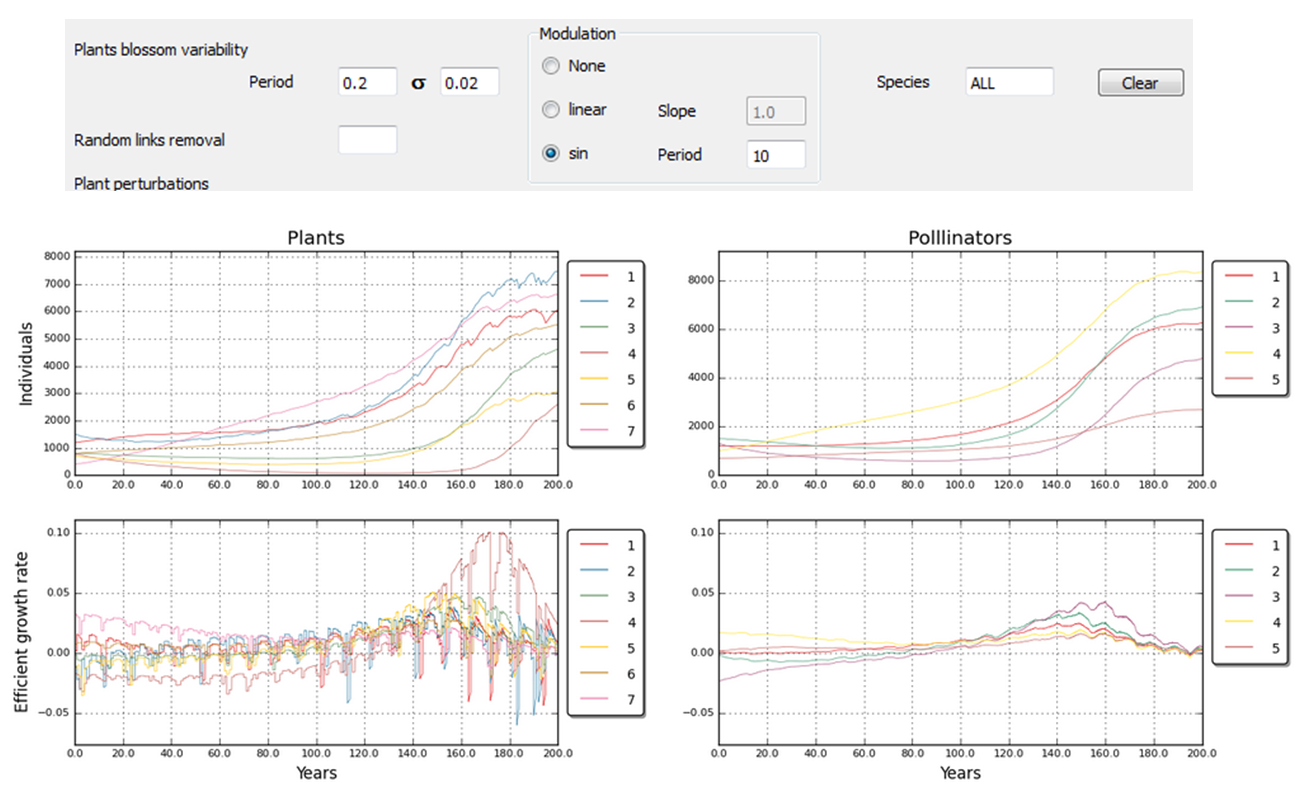
\includegraphics[scale=1]{ManFigs/sigmund_oscilacion_tiempo_sin.png}
\caption{Perturbación gaussiana en el periodo de floración con oscilación sinusoidal.}
\label{fig:ASIGMUNDMAN_sigmund_oscilacion_tiempo_sin}
\end{figure}

Para terminar estos ejemplos, una gráfica de la red ante aumentos abruptos pero breves de la mortalidad. En la figura \ref{fig:ASIGMUNDMAN_sigmund_95} se añade una mortalidad del $95\%$ durante $5$ años a la especie de polinizador $2$. La caída brusca está a punto de llevar a esta especie a la extinción pero al cesar el beneficio mutualista hace que se recupere porque no baja del mínimo vital aunque llega a estar muy próxima a él alrededor del año 90 de la simulación.

\begin{figure}[h!]
\centering
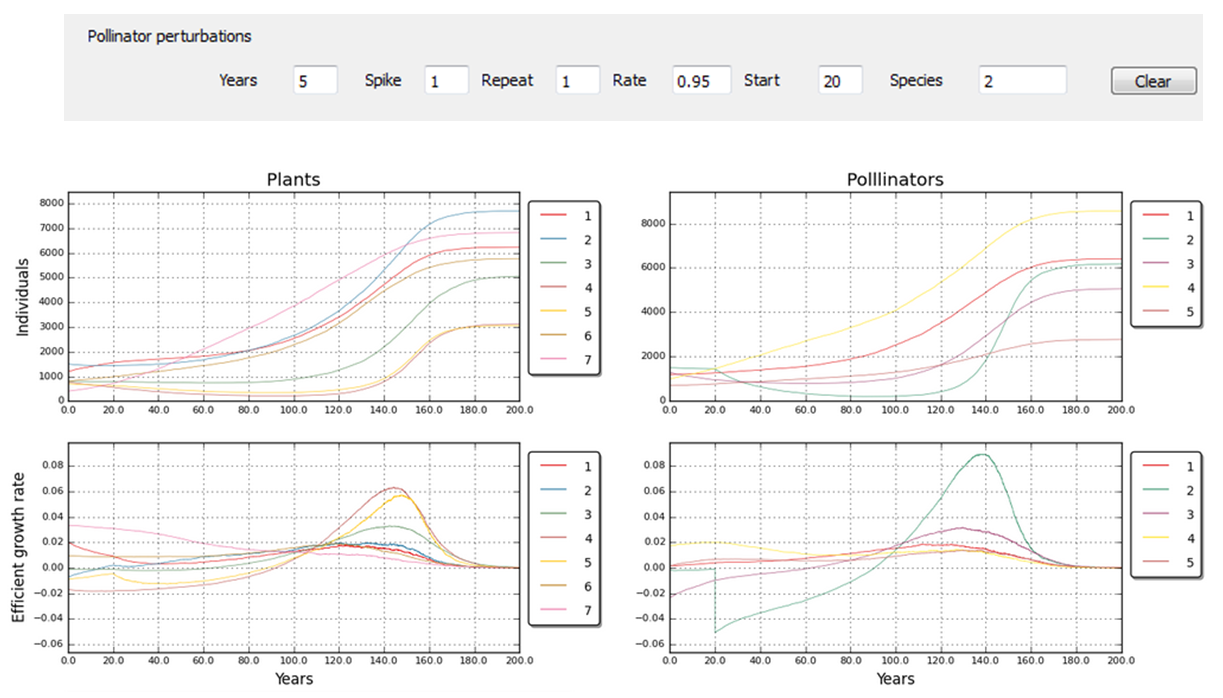
\includegraphics[scale=1]{ManFigs/sigmund_95.png}
\caption{Perturbación sobre la especie de polinizador .}
\label{fig:ASIGMUNDMAN_sigmund_95}
\end{figure}